\documentclass[]{article}
\usepackage{lmodern}
\usepackage{amssymb,amsmath}
\usepackage{ifxetex,ifluatex}
\usepackage{fixltx2e} % provides \textsubscript
\ifnum 0\ifxetex 1\fi\ifluatex 1\fi=0 % if pdftex
  \usepackage[T1]{fontenc}
  \usepackage[utf8]{inputenc}
\else % if luatex or xelatex
  \ifxetex
    \usepackage{mathspec}
  \else
    \usepackage{fontspec}
  \fi
  \defaultfontfeatures{Ligatures=TeX,Scale=MatchLowercase}
\fi
% use upquote if available, for straight quotes in verbatim environments
\IfFileExists{upquote.sty}{\usepackage{upquote}}{}
% use microtype if available
\IfFileExists{microtype.sty}{%
\usepackage{microtype}
\UseMicrotypeSet[protrusion]{basicmath} % disable protrusion for tt fonts
}{}
\usepackage[margin=1in]{geometry}
\usepackage{hyperref}
\hypersetup{unicode=true,
            pdftitle={Decorrelation methods and their effects on proposed method},
            pdfauthor={Xuelong Wang},
            pdfborder={0 0 0},
            breaklinks=true}
\urlstyle{same}  % don't use monospace font for urls
\usepackage{color}
\usepackage{fancyvrb}
\newcommand{\VerbBar}{|}
\newcommand{\VERB}{\Verb[commandchars=\\\{\}]}
\DefineVerbatimEnvironment{Highlighting}{Verbatim}{commandchars=\\\{\}}
% Add ',fontsize=\small' for more characters per line
\usepackage{framed}
\definecolor{shadecolor}{RGB}{248,248,248}
\newenvironment{Shaded}{\begin{snugshade}}{\end{snugshade}}
\newcommand{\KeywordTok}[1]{\textcolor[rgb]{0.13,0.29,0.53}{\textbf{#1}}}
\newcommand{\DataTypeTok}[1]{\textcolor[rgb]{0.13,0.29,0.53}{#1}}
\newcommand{\DecValTok}[1]{\textcolor[rgb]{0.00,0.00,0.81}{#1}}
\newcommand{\BaseNTok}[1]{\textcolor[rgb]{0.00,0.00,0.81}{#1}}
\newcommand{\FloatTok}[1]{\textcolor[rgb]{0.00,0.00,0.81}{#1}}
\newcommand{\ConstantTok}[1]{\textcolor[rgb]{0.00,0.00,0.00}{#1}}
\newcommand{\CharTok}[1]{\textcolor[rgb]{0.31,0.60,0.02}{#1}}
\newcommand{\SpecialCharTok}[1]{\textcolor[rgb]{0.00,0.00,0.00}{#1}}
\newcommand{\StringTok}[1]{\textcolor[rgb]{0.31,0.60,0.02}{#1}}
\newcommand{\VerbatimStringTok}[1]{\textcolor[rgb]{0.31,0.60,0.02}{#1}}
\newcommand{\SpecialStringTok}[1]{\textcolor[rgb]{0.31,0.60,0.02}{#1}}
\newcommand{\ImportTok}[1]{#1}
\newcommand{\CommentTok}[1]{\textcolor[rgb]{0.56,0.35,0.01}{\textit{#1}}}
\newcommand{\DocumentationTok}[1]{\textcolor[rgb]{0.56,0.35,0.01}{\textbf{\textit{#1}}}}
\newcommand{\AnnotationTok}[1]{\textcolor[rgb]{0.56,0.35,0.01}{\textbf{\textit{#1}}}}
\newcommand{\CommentVarTok}[1]{\textcolor[rgb]{0.56,0.35,0.01}{\textbf{\textit{#1}}}}
\newcommand{\OtherTok}[1]{\textcolor[rgb]{0.56,0.35,0.01}{#1}}
\newcommand{\FunctionTok}[1]{\textcolor[rgb]{0.00,0.00,0.00}{#1}}
\newcommand{\VariableTok}[1]{\textcolor[rgb]{0.00,0.00,0.00}{#1}}
\newcommand{\ControlFlowTok}[1]{\textcolor[rgb]{0.13,0.29,0.53}{\textbf{#1}}}
\newcommand{\OperatorTok}[1]{\textcolor[rgb]{0.81,0.36,0.00}{\textbf{#1}}}
\newcommand{\BuiltInTok}[1]{#1}
\newcommand{\ExtensionTok}[1]{#1}
\newcommand{\PreprocessorTok}[1]{\textcolor[rgb]{0.56,0.35,0.01}{\textit{#1}}}
\newcommand{\AttributeTok}[1]{\textcolor[rgb]{0.77,0.63,0.00}{#1}}
\newcommand{\RegionMarkerTok}[1]{#1}
\newcommand{\InformationTok}[1]{\textcolor[rgb]{0.56,0.35,0.01}{\textbf{\textit{#1}}}}
\newcommand{\WarningTok}[1]{\textcolor[rgb]{0.56,0.35,0.01}{\textbf{\textit{#1}}}}
\newcommand{\AlertTok}[1]{\textcolor[rgb]{0.94,0.16,0.16}{#1}}
\newcommand{\ErrorTok}[1]{\textcolor[rgb]{0.64,0.00,0.00}{\textbf{#1}}}
\newcommand{\NormalTok}[1]{#1}
\usepackage{graphicx,grffile}
\makeatletter
\def\maxwidth{\ifdim\Gin@nat@width>\linewidth\linewidth\else\Gin@nat@width\fi}
\def\maxheight{\ifdim\Gin@nat@height>\textheight\textheight\else\Gin@nat@height\fi}
\makeatother
% Scale images if necessary, so that they will not overflow the page
% margins by default, and it is still possible to overwrite the defaults
% using explicit options in \includegraphics[width, height, ...]{}
\setkeys{Gin}{width=\maxwidth,height=\maxheight,keepaspectratio}
\IfFileExists{parskip.sty}{%
\usepackage{parskip}
}{% else
\setlength{\parindent}{0pt}
\setlength{\parskip}{6pt plus 2pt minus 1pt}
}
\setlength{\emergencystretch}{3em}  % prevent overfull lines
\providecommand{\tightlist}{%
  \setlength{\itemsep}{0pt}\setlength{\parskip}{0pt}}
\setcounter{secnumdepth}{5}
% Redefines (sub)paragraphs to behave more like sections
\ifx\paragraph\undefined\else
\let\oldparagraph\paragraph
\renewcommand{\paragraph}[1]{\oldparagraph{#1}\mbox{}}
\fi
\ifx\subparagraph\undefined\else
\let\oldsubparagraph\subparagraph
\renewcommand{\subparagraph}[1]{\oldsubparagraph{#1}\mbox{}}
\fi

%%% Use protect on footnotes to avoid problems with footnotes in titles
\let\rmarkdownfootnote\footnote%
\def\footnote{\protect\rmarkdownfootnote}

%%% Change title format to be more compact
\usepackage{titling}

% Create subtitle command for use in maketitle
\newcommand{\subtitle}[1]{
  \posttitle{
    \begin{center}\large#1\end{center}
    }
}

\setlength{\droptitle}{-2em}

  \title{Decorrelation methods and their effects on proposed method}
    \pretitle{\vspace{\droptitle}\centering\huge}
  \posttitle{\par}
    \author{Xuelong Wang}
    \preauthor{\centering\large\emph}
  \postauthor{\par}
      \predate{\centering\large\emph}
  \postdate{\par}
    \date{2018-10-10}

\usepackage{float,amsmath, bbm, siunitx, bm}
\floatplacement{figure}{H}
\newcommand{\indep}{\rotatebox[origin=c]{90}{$\models$}}

\begin{document}
\maketitle

{
\setcounter{tocdepth}{2}
\tableofcontents
}
\section{Motivation}\label{motivation}

Based on the previous simulation result, we found that the decorrelation
step has a big influence on the final performance of the proposed
method. More specifically, when the \(n<p\) is happening then we known
that the sample covariance matrix \(\Sigma_{X}\) is not full rank.
Therefore, \(\Sigma^{-1}_X\), the inverse of \(\Sigma_{X}\), doesn't
exist. So we could calculate the general inverse of the covariance
matrix \(\Sigma_{X}\). In such situation, I just adapted one of commonly
used g-inverse -- the Moore penrose inverse \(\Sigma^{+}_X\) during the
decorrelation procedure. But the result is not very well compared with
the original method. Thus, the following is trying to discuss the reason
of why this is not working.

\section{SVD decorrelation procedure}\label{svd-decorrelation-procedure}

\[
  Var(X) = \Sigma_X = U\Lambda V^T,
\]

\begin{itemize}
\tightlist
\item
  \(X\) is the random vector with dim as \(p \times 1\),\\
\item
  \(\Sigma_X\) is \(p \times p\) symmetry matrix,\\
\item
  \(U = V\) are orthogonal matrix and each column is the eigenvector\\
\item
  \(\Lambda\) is a diagonal matrix with each diagonal element as the
  eigenvalue.
\end{itemize}

\subsection{\texorpdfstring{Assume the \(\Sigma_X\) is full
rank}{Assume the \textbackslash{}Sigma\_X is full rank}}\label{assume-the-sigma_x-is-full-rank}

To decorreate the X, we could just take the reciprocal of each square
root of eigenvalue as following.

\[
  \Sigma^{-\frac{1}{2}}_X = U\Lambda^{-\frac{1}{2}}U^T,
\] where
\(\Lambda^{-\frac{1}{2}} = \begin{bmatrix}  e_1^{-\frac{1}{2}} & \dots & 0 \\  \vdots & \ddots & \vdots \\  0 & \dots & e_p^{-\frac{1}{2}}  \end{bmatrix}\)

So that after transformation the \(\Sigma^{-\frac{1}{2}}_X X\) has
identity covariance matrix as following,

\[
  Var(\Sigma^{-\frac{1}{2}}_X X) = \Sigma^{-\frac{1}{2}}_X \Sigma_X\Sigma^{-\frac{1}{2}}_X = U\Lambda^{-\frac{1}{2}}U^T U\Lambda^{-1}U^T U\Lambda^{-\frac{1}{2}}U^T = I_p.
\]

\subsection{\texorpdfstring{Assume the \(\Sigma_X\) is not full
rank}{Assume the \textbackslash{}Sigma\_X is not full rank}}\label{assume-the-sigma_x-is-not-full-rank}

\[
  Var(X) = \Sigma_X = U\Lambda V^T =
                        \begin{bmatrix}
                         U_1 & U_2\\
                        \end{bmatrix}
                        \begin{bmatrix}
                        \Lambda_1 & 0\\
                        0 & 0
                        \end{bmatrix}
                        \begin{bmatrix}
                        U_1^T \\
                        U_2^T
                        \end{bmatrix} = U_1\Lambda_1U_1^T,
\] - \(U_1\) is a \(p \times r\) matrix with r \textless{} p and in most
of case r = n the sample size.

Then after applying the same procedure we get following,

\[
  \Sigma^{-\frac{1}{2}}_X = U_1\Lambda_1^{-\frac{1}{2}}U_1^T,
\] Note that in this case, I'm using Moore Penrose inverse.

After transformation the X we have, \[
  Var(\Sigma^{-\frac{1}{2}}_X X) = \Sigma^{-\frac{1}{2}}_X \Sigma_X\Sigma^{-\frac{1}{2}}_X = U_1\Lambda^{-\frac{1}{2}}_1U^T_1 U_1\Lambda^{-1}_1U^T_1 U_1\Lambda^{-\frac{1}{2}}_1U^T_1 = U_1U_1^T,  
\] Note that by the property of the U we have \[
  U_1U_1^T + U_2U_2^T = I_p, ~~~~~\\
  (U_1U_1^T)^T U_1U_1^T = U_1U_1^T,
\] Besides, \(U_1U_1^T\) and \(U_2U_2^T\) are indempotent and
\(rank(U_2U_2^T) + rank(U_1U_1^T) = p\).

So if the X is not full rank we cannot decorrelation the covariance
matrix to an identity matrix.

\subsection{Simulation stduy}\label{simulation-stduy}

\subsubsection{Simulation 1}\label{simulation-1}

\begin{Shaded}
\begin{Highlighting}[]
\CommentTok{# How the singular sample covariance affect the SVD decorrelation result}
\KeywordTok{set.seed}\NormalTok{(}\DecValTok{123}\NormalTok{)}
\NormalTok{p <-}\StringTok{ }\DecValTok{200}
\NormalTok{n <-}\StringTok{ }\DecValTok{200}
\NormalTok{Sig <-}\StringTok{ }\KeywordTok{matrix}\NormalTok{(}\KeywordTok{rep}\NormalTok{(}\FloatTok{0.5}\NormalTok{, }\DecValTok{200} \OperatorTok{*}\StringTok{ }\DecValTok{200}\NormalTok{), }\DataTypeTok{ncol =} \DecValTok{200}\NormalTok{)}
\KeywordTok{diag}\NormalTok{(Sig) <-}\StringTok{ }\DecValTok{1}
\NormalTok{x_total <-}\StringTok{ }\KeywordTok{mvrnorm}\NormalTok{(n, }\KeywordTok{numeric}\NormalTok{(p), }\DataTypeTok{Sigma =}\NormalTok{ Sig)}

\NormalTok{x_}\DecValTok{100}\NormalTok{ <-}\StringTok{ }\NormalTok{x_total[}\DecValTok{1}\OperatorTok{:}\DecValTok{100}\NormalTok{, ]}
\NormalTok{Est_sqrt_ins_cov_}\DecValTok{100}\NormalTok{ <-}\StringTok{ }\KeywordTok{invsqrt}\NormalTok{(}\KeywordTok{cov}\NormalTok{(x_}\DecValTok{100}\NormalTok{))}
\KeywordTok{cor}\NormalTok{(x_}\DecValTok{100} \OperatorTok\StringTok{ }\NormalTok{Est_sqrt_ins_cov_}\DecValTok{100}\NormalTok{)[}\DecValTok{1}\OperatorTok{:}\DecValTok{5}\NormalTok{, }\DecValTok{1}\OperatorTok{:}\DecValTok{5}\NormalTok{] }\OperatorTok\StringTok{ }\KeywordTok{round}\NormalTok{(., }\DecValTok{4}\NormalTok{)}
\OtherTok{FALSE}\NormalTok{         [,}\DecValTok{1}\NormalTok{]    [,}\DecValTok{2}\NormalTok{]    [,}\DecValTok{3}\NormalTok{]   [,}\DecValTok{4}\NormalTok{]    [,}\DecValTok{5}\NormalTok{]}
\OtherTok{FALSE}\NormalTok{ [}\DecValTok{1}\NormalTok{,]  }\FloatTok{1.0000} \OperatorTok{-}\FloatTok{0.0480} \OperatorTok{-}\FloatTok{0.0600} \FloatTok{0.0396} \OperatorTok{-}\FloatTok{0.0232}
\OtherTok{FALSE}\NormalTok{ [}\DecValTok{2}\NormalTok{,] }\OperatorTok{-}\FloatTok{0.0480}  \FloatTok{1.0000} \OperatorTok{-}\FloatTok{0.0339} \FloatTok{0.1562} \OperatorTok{-}\FloatTok{0.0701}
\OtherTok{FALSE}\NormalTok{ [}\DecValTok{3}\NormalTok{,] }\OperatorTok{-}\FloatTok{0.0600} \OperatorTok{-}\FloatTok{0.0339}  \FloatTok{1.0000} \FloatTok{0.0389} \OperatorTok{-}\FloatTok{0.0570}
\OtherTok{FALSE}\NormalTok{ [}\DecValTok{4}\NormalTok{,]  }\FloatTok{0.0396}  \FloatTok{0.1562}  \FloatTok{0.0389} \FloatTok{1.0000}  \FloatTok{0.0734}
\OtherTok{FALSE}\NormalTok{ [}\DecValTok{5}\NormalTok{,] }\OperatorTok{-}\FloatTok{0.0232} \OperatorTok{-}\FloatTok{0.0701} \OperatorTok{-}\FloatTok{0.0570} \FloatTok{0.0734}  \FloatTok{1.0000}
\KeywordTok{cor}\NormalTok{(x_}\DecValTok{100} \OperatorTok\StringTok{ }\NormalTok{Est_sqrt_ins_cov_}\DecValTok{100}\NormalTok{) }\OperatorTok\StringTok{ }\KeywordTok{abs}\NormalTok{(.) }\OperatorTok\StringTok{ }\KeywordTok{sum}\NormalTok{(.)}
\OtherTok{FALSE}\NormalTok{ [}\DecValTok{1}\NormalTok{] }\FloatTok{2480.243}
\KeywordTok{cov}\NormalTok{(x_}\DecValTok{100} \OperatorTok\StringTok{ }\NormalTok{Est_sqrt_ins_cov_}\DecValTok{100}\NormalTok{) }\OperatorTok\StringTok{ }\KeywordTok{diag}\NormalTok{(.) }\OperatorTok\StringTok{ }\KeywordTok{sum}\NormalTok{(.)}
\OtherTok{FALSE}\NormalTok{ [}\DecValTok{1}\NormalTok{] }\DecValTok{99}
\KeywordTok{cor}\NormalTok{(x_}\DecValTok{100} \OperatorTok\StringTok{ }\NormalTok{Est_sqrt_ins_cov_}\DecValTok{100}\NormalTok{)[}\KeywordTok{cor}\NormalTok{(x_}\DecValTok{100} \OperatorTok\StringTok{ }\NormalTok{Est_sqrt_ins_cov_}\DecValTok{100}\NormalTok{) }\OperatorTok\StringTok{ }
\StringTok{    }\KeywordTok{lower.tri}\NormalTok{(., }\DataTypeTok{diag =} \OtherTok{FALSE}\NormalTok{)] }\OperatorTok\StringTok{ }\KeywordTok{max}\NormalTok{()}
\OtherTok{FALSE}\NormalTok{ [}\DecValTok{1}\NormalTok{] }\FloatTok{0.2839148}

\NormalTok{x_}\DecValTok{200}\NormalTok{ <-}\StringTok{ }\NormalTok{x_total}
\NormalTok{Est_sqrt_ins_cov_}\DecValTok{200}\NormalTok{ <-}\StringTok{ }\KeywordTok{invsqrt}\NormalTok{(}\KeywordTok{cov}\NormalTok{(x_}\DecValTok{200}\NormalTok{))}
\KeywordTok{cor}\NormalTok{(x_}\DecValTok{200} \OperatorTok\StringTok{ }\NormalTok{Est_sqrt_ins_cov_}\DecValTok{200}\NormalTok{)[}\DecValTok{1}\OperatorTok{:}\DecValTok{5}\NormalTok{, }\DecValTok{1}\OperatorTok{:}\DecValTok{5}\NormalTok{] }\OperatorTok\StringTok{ }\KeywordTok{round}\NormalTok{(., }\DecValTok{4}\NormalTok{)}
\OtherTok{FALSE}\NormalTok{         [,}\DecValTok{1}\NormalTok{]    [,}\DecValTok{2}\NormalTok{]    [,}\DecValTok{3}\NormalTok{]   [,}\DecValTok{4}\NormalTok{]    [,}\DecValTok{5}\NormalTok{]}
\OtherTok{FALSE}\NormalTok{ [}\DecValTok{1}\NormalTok{,]  }\FloatTok{1.0000}  \FloatTok{0.0032}  \FloatTok{0.0024} \OperatorTok{-}\FloatTok{3e-04}  \FloatTok{0.0034}
\OtherTok{FALSE}\NormalTok{ [}\DecValTok{2}\NormalTok{,]  }\FloatTok{0.0032}  \FloatTok{1.0000} \OperatorTok{-}\FloatTok{0.0049}  \FloatTok{6e-04} \OperatorTok{-}\FloatTok{0.0069}
\OtherTok{FALSE}\NormalTok{ [}\DecValTok{3}\NormalTok{,]  }\FloatTok{0.0024} \OperatorTok{-}\FloatTok{0.0049}  \FloatTok{1.0000}  \FloatTok{4e-04} \OperatorTok{-}\FloatTok{0.0052}
\OtherTok{FALSE}\NormalTok{ [}\DecValTok{4}\NormalTok{,] }\OperatorTok{-}\FloatTok{0.0003}  \FloatTok{0.0006}  \FloatTok{0.0004}  \FloatTok{1e+00}  \FloatTok{0.0006}
\OtherTok{FALSE}\NormalTok{ [}\DecValTok{5}\NormalTok{,]  }\FloatTok{0.0034} \OperatorTok{-}\FloatTok{0.0069} \OperatorTok{-}\FloatTok{0.0052}  \FloatTok{6e-04}  \FloatTok{1.0000}
\KeywordTok{cor}\NormalTok{(x_}\DecValTok{200} \OperatorTok\StringTok{ }\NormalTok{Est_sqrt_ins_cov_}\DecValTok{200}\NormalTok{) }\OperatorTok\StringTok{ }\KeywordTok{abs}\NormalTok{(.) }\OperatorTok\StringTok{ }\KeywordTok{sum}\NormalTok{(.)}
\OtherTok{FALSE}\NormalTok{ [}\DecValTok{1}\NormalTok{] }\FloatTok{327.6482}
\KeywordTok{cov}\NormalTok{(x_}\DecValTok{200} \OperatorTok\StringTok{ }\NormalTok{Est_sqrt_ins_cov_}\DecValTok{200}\NormalTok{) }\OperatorTok\StringTok{ }\KeywordTok{diag}\NormalTok{(.) }\OperatorTok\StringTok{ }\KeywordTok{sum}\NormalTok{(.)}
\OtherTok{FALSE}\NormalTok{ [}\DecValTok{1}\NormalTok{] }\DecValTok{199}
\KeywordTok{cor}\NormalTok{(x_}\DecValTok{200} \OperatorTok\StringTok{ }\NormalTok{Est_sqrt_ins_cov_}\DecValTok{200}\NormalTok{)[}\KeywordTok{cor}\NormalTok{(x_}\DecValTok{200} \OperatorTok\StringTok{ }\NormalTok{Est_sqrt_ins_cov_}\DecValTok{200}\NormalTok{) }\OperatorTok\StringTok{ }
\StringTok{    }\KeywordTok{lower.tri}\NormalTok{(., }\DataTypeTok{diag =} \OtherTok{FALSE}\NormalTok{)] }\OperatorTok\StringTok{ }\KeywordTok{max}\NormalTok{()}
\OtherTok{FALSE}\NormalTok{ [}\DecValTok{1}\NormalTok{] }\FloatTok{0.03669759}

\CommentTok{# if we use the inverse information of x_200}
\KeywordTok{cor}\NormalTok{(x_}\DecValTok{100} \OperatorTok\StringTok{ }\NormalTok{Est_sqrt_ins_cov_}\DecValTok{200}\NormalTok{)[}\DecValTok{1}\OperatorTok{:}\DecValTok{5}\NormalTok{, }\DecValTok{1}\OperatorTok{:}\DecValTok{5}\NormalTok{] }\OperatorTok\StringTok{ }\KeywordTok{round}\NormalTok{(., }\DecValTok{4}\NormalTok{)}
\OtherTok{FALSE}\NormalTok{         [,}\DecValTok{1}\NormalTok{]    [,}\DecValTok{2}\NormalTok{]    [,}\DecValTok{3}\NormalTok{]    [,}\DecValTok{4}\NormalTok{]    [,}\DecValTok{5}\NormalTok{]}
\OtherTok{FALSE}\NormalTok{ [}\DecValTok{1}\NormalTok{,]  }\FloatTok{1.0000} \OperatorTok{-}\FloatTok{0.0065} \OperatorTok{-}\FloatTok{0.1252} \OperatorTok{-}\FloatTok{0.0091} \OperatorTok{-}\FloatTok{0.0865}
\OtherTok{FALSE}\NormalTok{ [}\DecValTok{2}\NormalTok{,] }\OperatorTok{-}\FloatTok{0.0065}  \FloatTok{1.0000} \OperatorTok{-}\FloatTok{0.0076}  \FloatTok{0.2172} \OperatorTok{-}\FloatTok{0.0999}
\OtherTok{FALSE}\NormalTok{ [}\DecValTok{3}\NormalTok{,] }\OperatorTok{-}\FloatTok{0.1252} \OperatorTok{-}\FloatTok{0.0076}  \FloatTok{1.0000}  \FloatTok{0.0741} \OperatorTok{-}\FloatTok{0.0986}
\OtherTok{FALSE}\NormalTok{ [}\DecValTok{4}\NormalTok{,] }\OperatorTok{-}\FloatTok{0.0091}  \FloatTok{0.2172}  \FloatTok{0.0741}  \FloatTok{1.0000}  \FloatTok{0.0489}
\OtherTok{FALSE}\NormalTok{ [}\DecValTok{5}\NormalTok{,] }\OperatorTok{-}\FloatTok{0.0865} \OperatorTok{-}\FloatTok{0.0999} \OperatorTok{-}\FloatTok{0.0986}  \FloatTok{0.0489}  \FloatTok{1.0000}
\KeywordTok{cor}\NormalTok{(x_}\DecValTok{100} \OperatorTok\StringTok{ }\NormalTok{Est_sqrt_ins_cov_}\DecValTok{200}\NormalTok{) }\OperatorTok\StringTok{ }\KeywordTok{abs}\NormalTok{(.) }\OperatorTok\StringTok{ }\KeywordTok{sum}\NormalTok{(.)}
\OtherTok{FALSE}\NormalTok{ [}\DecValTok{1}\NormalTok{] }\FloatTok{2479.92}
\KeywordTok{cov}\NormalTok{(x_}\DecValTok{100} \OperatorTok\StringTok{ }\NormalTok{Est_sqrt_ins_cov_}\DecValTok{200}\NormalTok{) }\OperatorTok\StringTok{ }\KeywordTok{diag}\NormalTok{(.) }\OperatorTok\StringTok{ }\KeywordTok{sum}\NormalTok{(.)}
\OtherTok{FALSE}\NormalTok{ [}\DecValTok{1}\NormalTok{] }\DecValTok{199}
\KeywordTok{cor}\NormalTok{(x_}\DecValTok{100} \OperatorTok\StringTok{ }\NormalTok{Est_sqrt_ins_cov_}\DecValTok{200}\NormalTok{)[}\KeywordTok{cor}\NormalTok{(x_}\DecValTok{100} \OperatorTok\StringTok{ }\NormalTok{Est_sqrt_ins_cov_}\DecValTok{200}\NormalTok{) }\OperatorTok\StringTok{ }
\StringTok{    }\KeywordTok{lower.tri}\NormalTok{(., }\DataTypeTok{diag =} \OtherTok{FALSE}\NormalTok{)] }\OperatorTok\StringTok{ }\KeywordTok{max}\NormalTok{()}
\OtherTok{FALSE}\NormalTok{ [}\DecValTok{1}\NormalTok{] }\FloatTok{0.2662189}
\end{Highlighting}
\end{Shaded}

\begin{itemize}
\tightlist
\item
  As we expected, when \(n < p\), SVD decorrelation's result is not as
  good as full rank case ( \(n\geq p\)), which means off diagonal
  elements are not equal or closed to zero
\item
  The largest correlation coefficient of \(X_{100}\) is 0.28 and the for
  \(X_{200}\) is 0.0036
\item
  If we use the sample variance of \(X_{200}\) to decorrelate
  \(X_{100}\), it seems there is a little improvement on the max
  correlation coefficient
\end{itemize}

\subsubsection{Simulation 2}\label{simulation-2}

Next, I tried to evaluate the performance of the GCTA and proposed
method under the \(n < p\) scenario. To keep the problem simple, I just
let the covariates to be independent to each other. We want to see if
the original GCTA method is affected by the singular sample covariance
matrix problem. If it was able to work fine, then it verify the proposed
method. More specifically, If we could find a linear transformation on
covariates X to make them independent or un-correlated at least in
population level (although we still have the singular sample covariance
matrix problem), then we could still get a unbiased estimation of the
total covariates variance.

\paragraph{A toy sample}\label{a-toy-sample}

\begin{Shaded}
\begin{Highlighting}[]
\NormalTok{x <-}\StringTok{ }\KeywordTok{mvrnorm}\NormalTok{(}\DecValTok{100}\NormalTok{, }\KeywordTok{numeric}\NormalTok{(}\DecValTok{200}\NormalTok{), }\KeywordTok{diag}\NormalTok{(}\DecValTok{200}\NormalTok{))}
\KeywordTok{cor}\NormalTok{(x) }\OperatorTok\StringTok{ }\KeywordTok{abs}\NormalTok{(.) }\OperatorTok\StringTok{ }\KeywordTok{sum}\NormalTok{(.)}
\OtherTok{FALSE}\NormalTok{ [}\DecValTok{1}\NormalTok{] }\FloatTok{3412.224}
\KeywordTok{max}\NormalTok{(}\KeywordTok{cor}\NormalTok{(x)[}\KeywordTok{lower.tri}\NormalTok{(}\KeywordTok{cor}\NormalTok{(x))])}
\OtherTok{FALSE}\NormalTok{ [}\DecValTok{1}\NormalTok{] }\FloatTok{0.3585155}
\end{Highlighting}
\end{Shaded}

\begin{itemize}
\tightlist
\item
  this is to show that although the covariates are independent in
  population level, their sample correlation may still be large
\item
  the GCTA method may be effected by the this problem or not
\end{itemize}

\paragraph{Simulation set up}\label{simulation-set-up}

\[
  X = [x_1^2, \dots, x_p^2]^T
\]

\begin{itemize}
\tightlist
\item
  \(p = 34\)\\
\item
  \(x_i \stackrel{iid}{\sim} N(0,1)\)\\
\item
  So \(x_i^2\) are iid chi-square with \(df = 1\)
\end{itemize}

We consider to estimate the total variance, so that the total covariates
(combined main and interaction terms) is 595. Let the sample size n
increase from 100 to 600 in order to see how the \(p < n\) simulation
affect the GCTA and proposed method's performance. Following is the
simulation result.

\paragraph{Simulation results}\label{simulation-results}

\begin{figure}
\centering
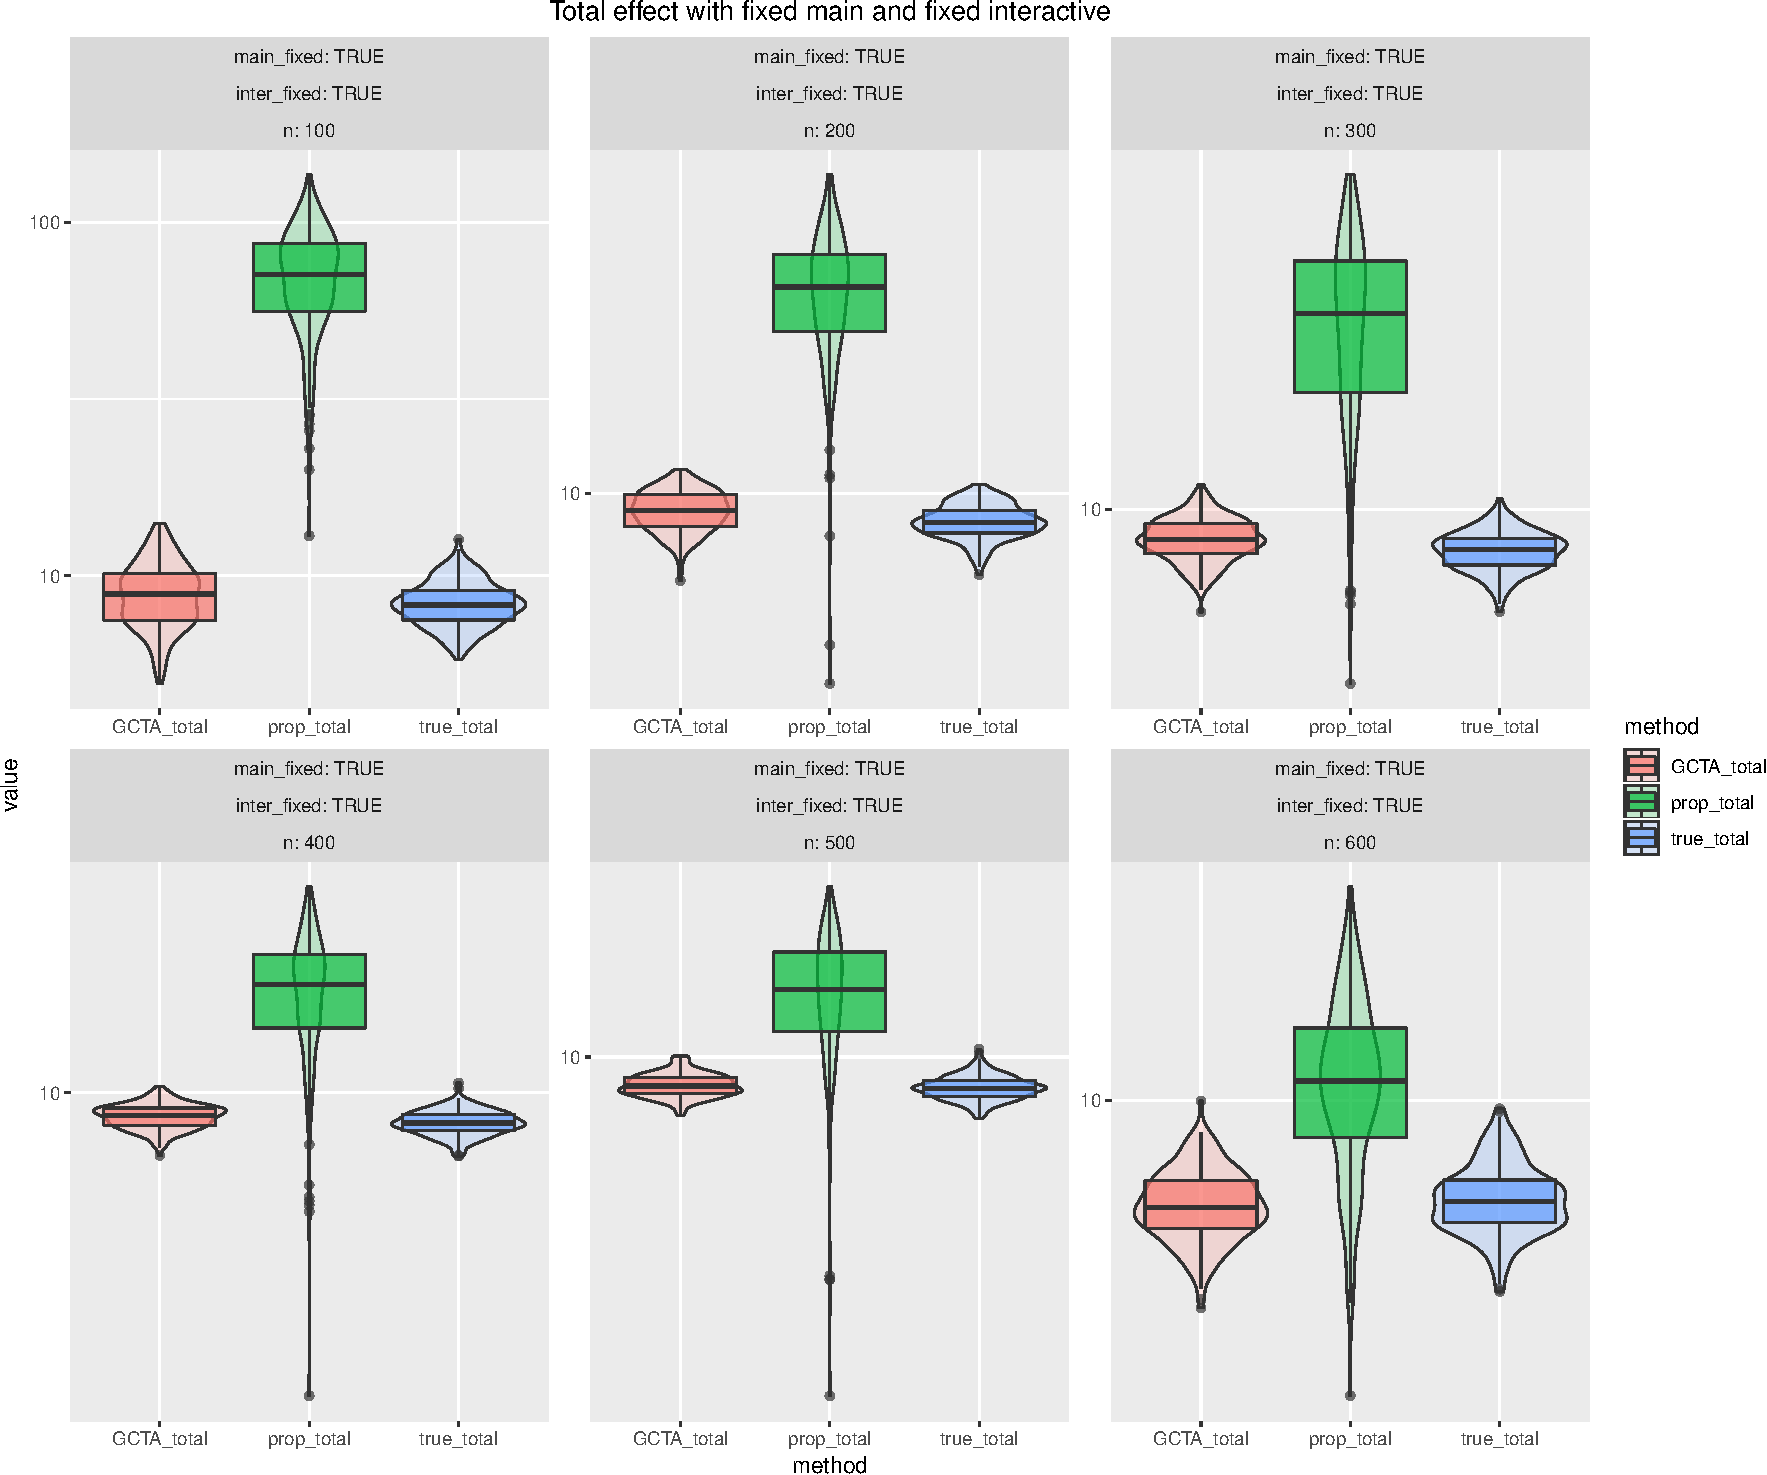
\includegraphics{Decorrelation_method_and_their_effect_on_proposed_method_files/figure-latex/fixed_fixed-1.pdf}
\caption{Fixed\_Fixed total independet chi with df = 1}
\end{figure}

\begin{figure}
\centering
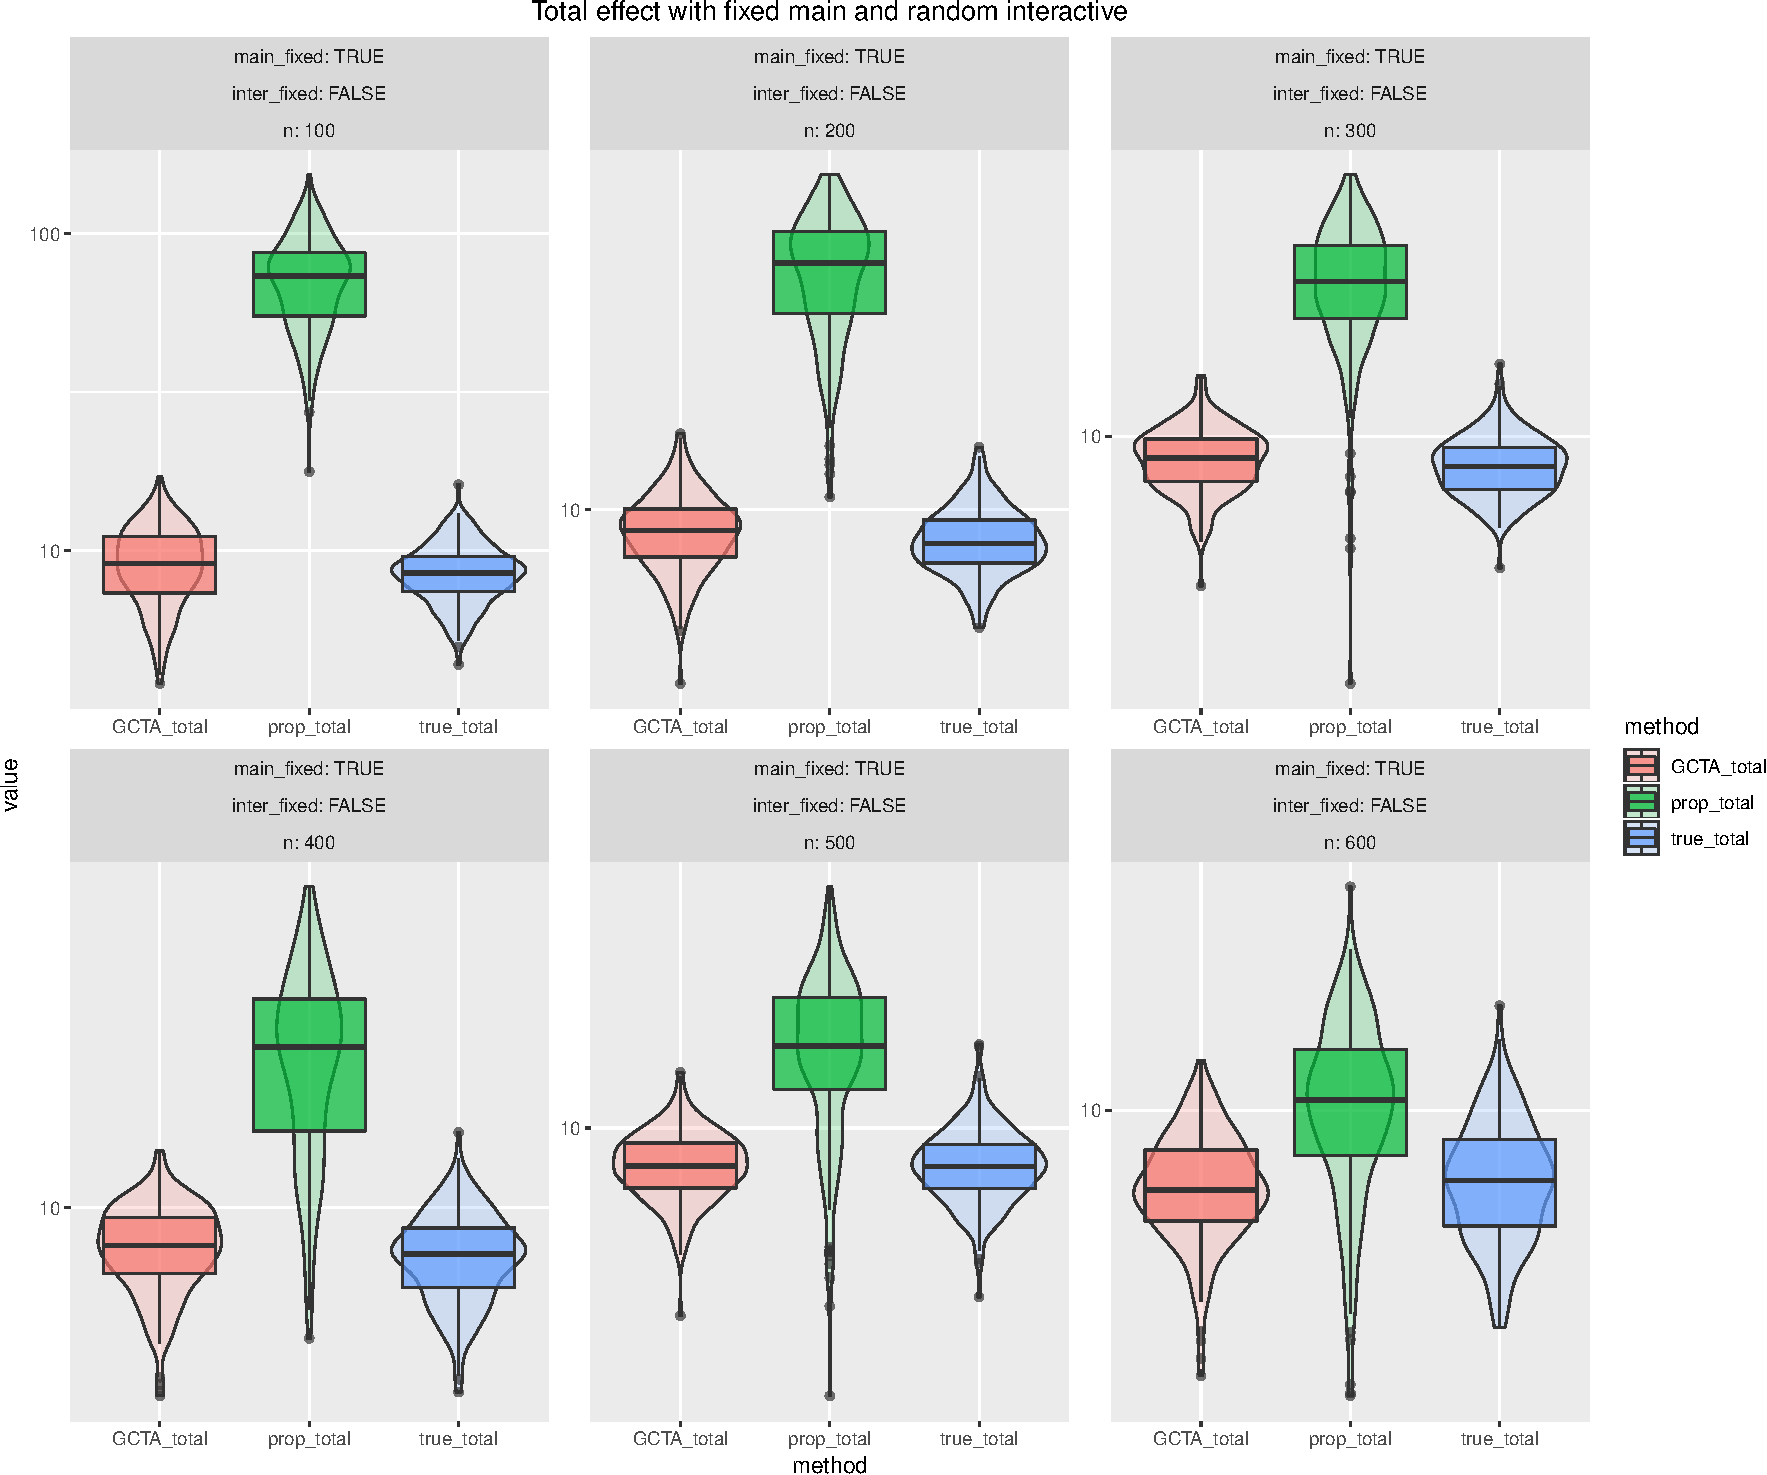
\includegraphics{Decorrelation_method_and_their_effect_on_proposed_method_files/figure-latex/fixed_random-1.pdf}
\caption{fixed\_random total independet chi with df = 1}
\end{figure}

\begin{figure}
\centering
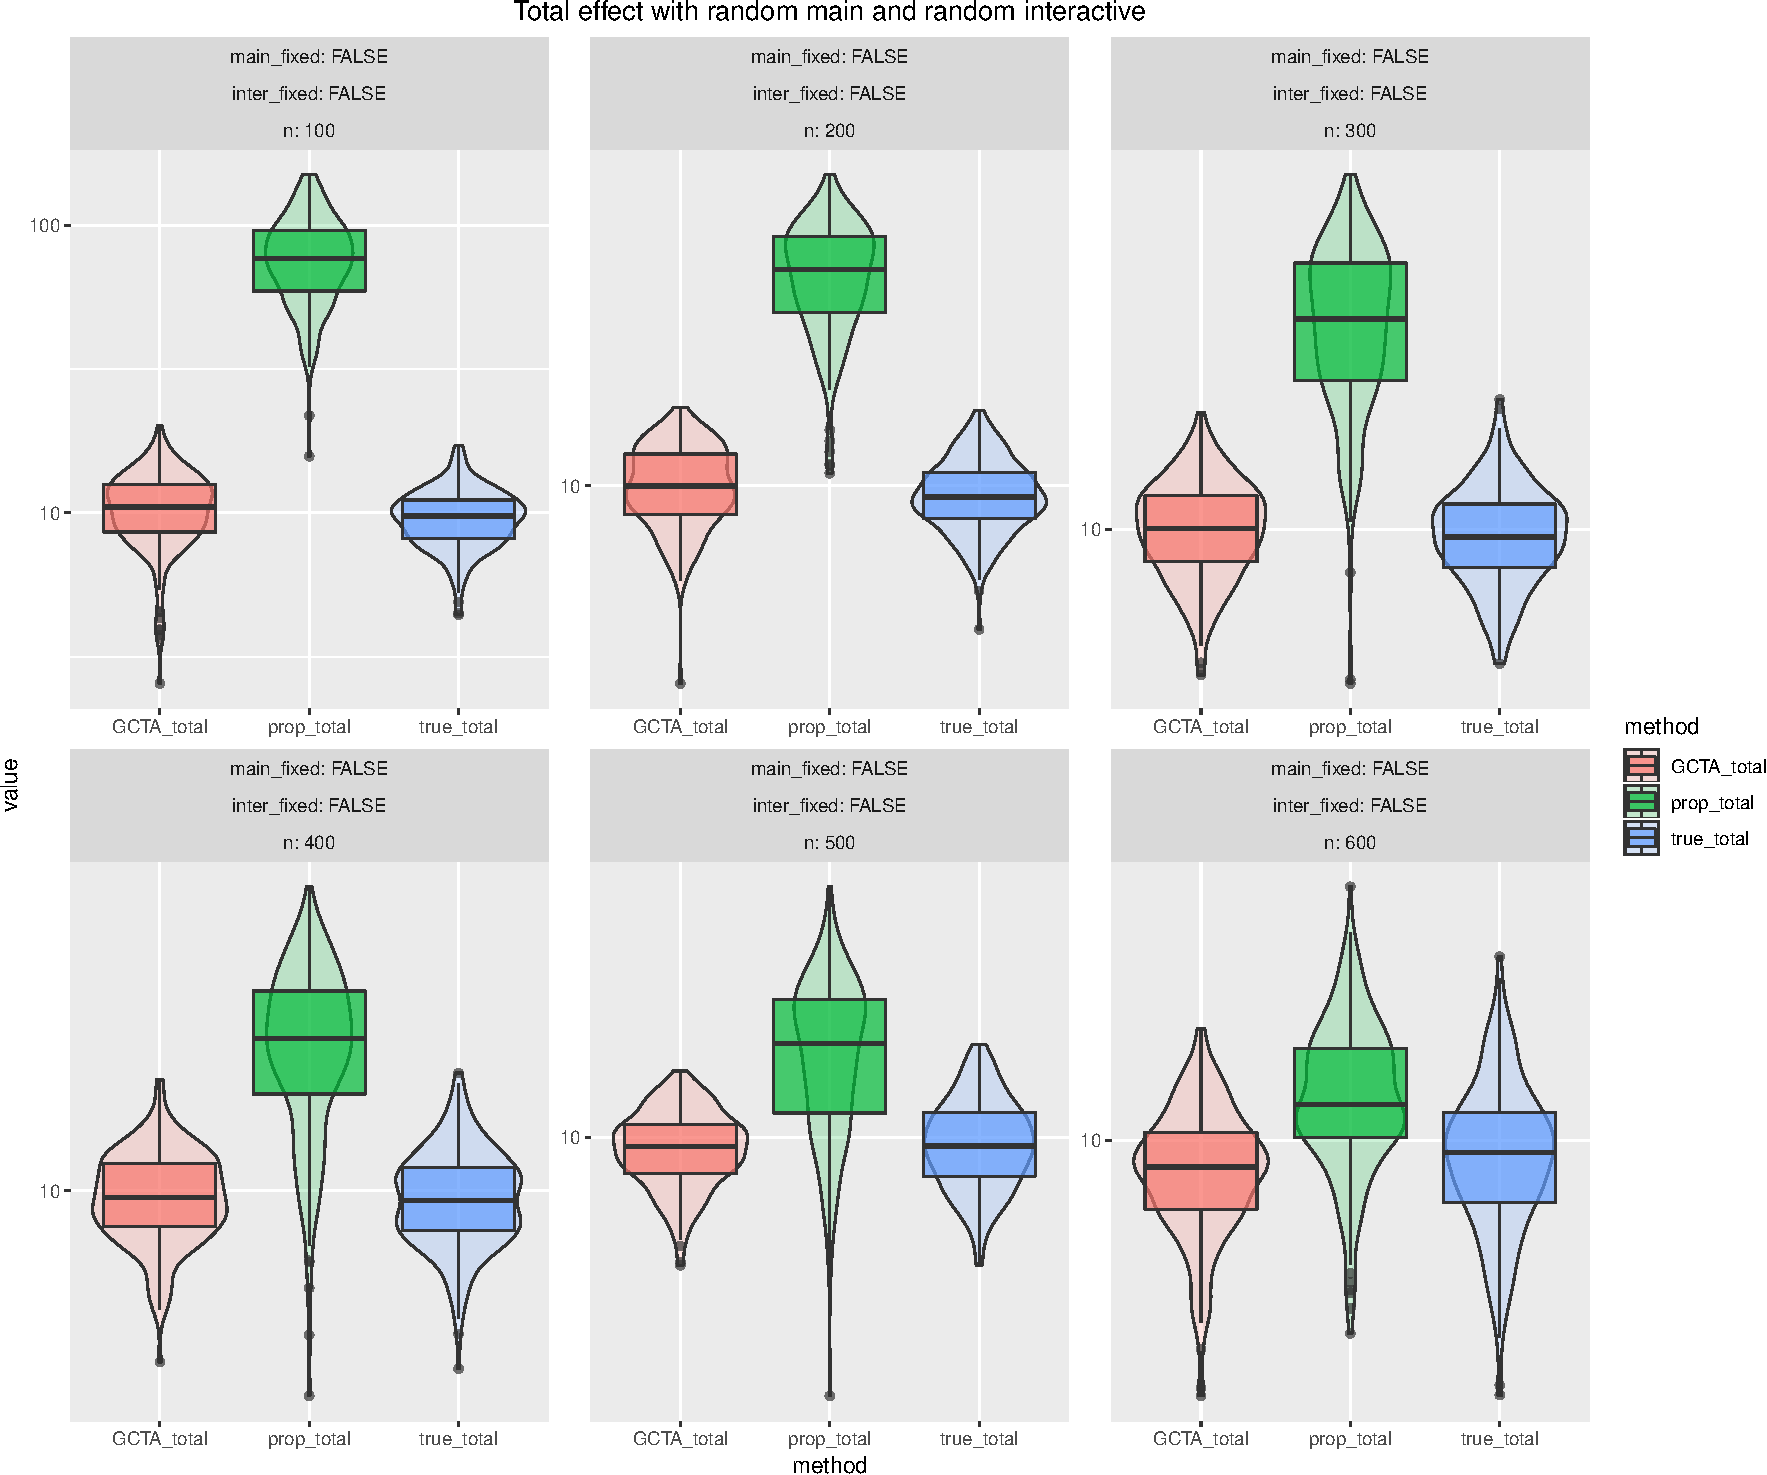
\includegraphics{Decorrelation_method_and_their_effect_on_proposed_method_files/figure-latex/random_random-1.pdf}
\caption{random\_random total independet chi with df = 1}
\end{figure}

\begin{itemize}
\tightlist
\item
  The original GCTA method is not affected by the \(p < n\) condition if
  the covariates are independent in the population level
\item
  note that actual the covariates are not perfectly independent because
  of the interaction terms
\item
  the proposed method is affected a lot by the \(p <n\) situation, but
  it getting better when sample size is increasing
\end{itemize}

\section{Lasso regression decorrelation
procedure}\label{lasso-regression-decorrelation-procedure}

\subsection{Motivation}\label{motivation-1}

Based on the previous result, we find that the original GCTA is not
sensitive to the \(p < n\) situation. So the next question is to find a
way to decorrelating the covariates so that they become uncorrelated in
the population level. The SVD method seems not work well in that
situation as previous simulations shows. Therefore, we look for the
lasso regression method.

\subsection{Main Idea and step}\label{main-idea-and-step}

The main idea of lasso regression is to find a procedure of
decorrelation. we could consider each covaraite as the dependent
variable and select several other covariates as the independent
variables. Then, we could preformance a lasso regression and use the
residual as the new covariates. After doing that the residuals should be
uncorrelated to each other.

\[
  X = [X_1, \dots X_p]
\]

\begin{itemize}
\tightlist
\item
  X is a \(n \times p\) observed covariates matrix
\item
  \(X_i, ~~ i = 1, \dots, p\) are the columns of X
\end{itemize}

\begin{enumerate}
\def\labelenumi{\arabic{enumi}.}
\tightlist
\item
  For each \(X_i\), select a group \(\mathcal{A}_t\) of variable as the
  independent variable
\item
  Conduct lasso regression and decide the final group of active
  variables as the independent variables \(\mathcal{A}_f\), note that
  \(\mathcal{A}_f \subset \mathcal{A}_t\)
\item
  Conduct a linear regression with
  \(Y = X_i ~~ X = X_j, j\in\mathcal{A}_f\) and use the residual as the
  new covariate \(Z_i = X_i - \hat{X_i}\)
\end{enumerate}

\section{Sigularity of the sample covariance
matrix}\label{sigularity-of-the-sample-covariance-matrix}

Based on the simulation study, the results suggest that the proposed
method has a bias in total (ultimate) effect estimation when \(n<p\)
situation. One of the most relative reason is that the way we used to
estimate the sample covariance matrix. We suspect that the singularity
of the sample covariance (Note its
\(rank \leq p-1, because it using sample mean to calculate the sample covariance\))
affects the result the proposed method.

\subsection{\texorpdfstring{Solution 1, using SVD to reduce the total
covariate matrix into a \(n \times n\)
matrix}{Solution 1, using SVD to reduce the total covariate matrix into a n \textbackslash{}times n matrix}}\label{solution-1-using-svd-to-reduce-the-total-covariate-matrix-into-a-n-times-n-matrix}

\subsubsection{Main idea}\label{main-idea}

\[
  X = U \Sigma V^T = \begin{bmatrix}
                      U_1 & U_2
                      \end{bmatrix}
                      \begin{bmatrix}
                      \Lambda_1 & 0\\
                      0 & 0
                      \end{bmatrix}
                      \begin{bmatrix}
                      V_1 & V_2\\
                      V_3 & V_4
                      \end{bmatrix}^T 
                      = 
                      \begin{bmatrix}
                      U_1 & U_2
                      \end{bmatrix}
                      \begin{bmatrix} 
\]


\end{document}
